\documentclass[a4paper, 11pt]{article}

%Comandos para configurar el idioma
\usepackage[spanish,activeacute]{babel}
\usepackage[utf8]{inputenc}
\usepackage[T1]{fontenc} %Necesario para el uso de las comillas latinas.
\usepackage{geometry}
\usepackage{graphicx}

%Importante que esta sea la última órden del preámbulo
\usepackage{hyperref}

\newcommand\fnurl[2]{%
  \href{#2}{#1}\footnote{\url{#2}}%
}

%Paquetes matemáticos
\usepackage{amsmath,amsfonts,amsthm}
\usepackage[all]{xy} %Para diagramas
\usepackage{enumerate} %Personalización de enumeraciones
\usepackage{tikz} %Dibujos

%Tipografía escalable
\usepackage{lmodern}
%Legibilidad
\usepackage{microtype}

%Código
\usepackage{listings}
\usepackage{color}

\definecolor{dkgreen}{rgb}{0,0.6,0}
\definecolor{gray}{rgb}{0.5,0.5,0.5}
\definecolor{mauve}{rgb}{0.58,0,0.82}

\definecolor{listinggray}{gray}{0.9}
\definecolor{lbcolor}{rgb}{0.9,0.9,0.9}
\lstset{
backgroundcolor=\color{lbcolor},
    tabsize=4,
rulecolor=,
    language=[GNU]C++,
        basicstyle=\scriptsize,
        upquote=true,
        aboveskip={1.5\baselineskip},
        columns=fixed,
        showstringspaces=false,
        extendedchars=false,
        breaklines=true,
        prebreak = \raisebox{0ex}[0ex][0ex]{\ensuremath{\hookleftarrow}},
        frame=single,
        numbers=left,
        showtabs=false,
        showspaces=false,
        showstringspaces=false,
        identifierstyle=\ttfamily,
        keywordstyle=\color[rgb]{0,0,1},
        commentstyle=\color[rgb]{0.026,0.112,0.095},
        stringstyle=\color[rgb]{0.627,0.126,0.941},
        numberstyle=\color[rgb]{0.205, 0.142, 0.73},
%        \lstdefinestyle{C++}{language=C++,style=numbers}’.
}
\lstset{
    backgroundcolor=\color{lbcolor},
    tabsize=4,
  language=C++,
  captionpos=b,
  tabsize=3,
  frame=lines,
  numbers=left,
  numberstyle=\tiny,
  numbersep=5pt,
  breaklines=true,
  showstringspaces=false,
  basicstyle=\footnotesize,
%  identifierstyle=\color{magenta},
  keywordstyle=\color[rgb]{0,0,1},
  commentstyle=\color[rgb]{0.026,0.112,0.095}, % Darkgreen
  stringstyle=\color{red}
  }
% Slightly bigger margins than the latex defaults

\geometry{verbose,tmargin=1in,bmargin=1in,lmargin=1in,rmargin=1in}

\theoremstyle{definition}
\newtheorem{ejercicio}{Ejercicio}
\newtheorem{cuestion}{Cuestión}
\newtheorem*{solucion}{Solución}
\newtheorem*{bonus}{BONUS}

%%%%%%%% New sqrt
\usepackage{letltxmacro}
\makeatletter
\let\oldr@@t\r@@t
\def\r@@t#1#2{%
\setbox0=\hbox{$\oldr@@t#1{#2\,}$}\dimen0=\ht0
\advance\dimen0-0.2\ht0
\setbox2=\hbox{\vrule height\ht0 depth -\dimen0}%
{\box0\lower0.4pt\box2}}
\LetLtxMacro{\oldsqrt}{\sqrt}
\renewcommand*{\sqrt}[2][\ ]{\oldsqrt[#1]{#2} }
\makeatother

%%%%%%%%%%%%%%%%%%%%%%%%%%%%%%%%%%%%%%%%%%%

\hypersetup{
  pdftitle={Informe de trabajo 1},
  pdfauthor={Antonio Álvarez Caballero},
  unicode,
  breaklinks=true,  % so long urls are correctly broken across lines
  colorlinks=true,
  urlcolor=blue,
  linkcolor=darkorange,
  citecolor=darkgreen,
  }

\title{Informe de trabajo 1}
\author{Antonio Álvarez Caballero\\
    \href{mailto:analca3@correo.ugr.es}{analca3@correo.ugr.es}}
\date{}
%%%%%%%%%%%%%%%%% FIN PREAMBULO %%%%%%%%%%%%%%%%%%%%%%%%%%%

\begin{document}

  \maketitle

  \section{Convolución}

  La primera parte de la práctica consiste en aplicar un filtro de convolución
  (en este caso, un filtro de alisamiento Gaussiano) a una imagen. Para ello,
  partiendo de la función Gaussiana en una sola variable (recordamos que este filtro
  es separable en filas y columnas), realizaremos una serie de pasos.

  \subsection{Creación del vector máscara}

  El primero de ellos será, a partir de la función proporcionada $f(x)=exp(-0.5\frac{x^2}{\sigma^2})$
  y de un valor $\sigma$ , generar un vector máscara representativo. Para conseguirlo,
  debemos recordar que para que la máscara sea significativa debe contener la región
  $[-3\sigma,3\sigma]$. Sabiendo esto, la longitud de la máscara podremos conseguirla
  aplicando en \textit{C++} esta operación:
  es

  \begin{lstlisting}
    float dimension = 2*round(3*sigma) + 1;
  \end{lstlisting}

  ¿Por qué? Pues porque así conseguimos discretizar $3\sigma$ y que la máscara
  tenga en ambos lados dicha longitud. Luego sumamos $1$ para contar también el centro.\\

  Una vez tenemos la dimensión de la máscara, debemos aplicar $f(x)$ a los índices
  de nuestra máscara. Es decir, para $\sigma = 1$, la dimensión sería $7$, y los
  índices de la máscara $[-3,-2,-1,0,1,2,3]$, pues debemos aplicar $f(x)$ a dichos
  valores para obtener nuestro vector máscara. No debemos olvidarnos de normalizar
  la máscara como último paso.

  \begin{lstlisting}
    Mat Image::gaussianMask(float sigma)
    {
      int mask_size = 2 * round(3 * sigma) + 1; // +-3*sigma plus the zero
      int mask_center = round(3 * sigma);

      float value = 0, sum_values = 0;
      int mask_index;

      Mat mask = Mat::zeros(1, mask_size, CV_32FC1);

      for (int i = 0; i < mask_size; i++)
      {
        mask_index = i - mask_center;
        value = exp(-0.5 * (mask_index * mask_index) / (sigma * sigma));

        mask.at<float>(Point(i,0)) = value;
        sum_values += value;
      }

      mask *= 1.0 / sum_values;

      return mask;
    }
  \end{lstlisting}

  \subsection{Aplicación del vector máscara sobre una fila}

  El siguiente paso es aplicar dicha máscara sobre un vector fila. Para ello, debemos
  expandir el vector de entrada (a partir de ahora, vector señal) para poder tomar
  algún píxel vecino a los de los extremos de la imagen, para poder pasar por ellos también
  la máscara. En este caso hemos trabajado con los modos \textit{Reflejado} y \textit{Constante}.
  Para ello hemos utilizado la función de OpenCV \textit{copyMakeBorder}, que es
  muy versátil y nos permite copiar una imagen en otra con un determinado borde.
  Nos permite también decidir el modo de expansión que queremos, que en nuestro caso,
  como hemos indicado, son \textit{Reflejado} y \textit{Constante}.\\

  La lógica es la siguiente: expandimos la imagen, y luego, vamos extrayendo
  un ROI del mismo tamaño de la máscara por todo el vector, realizando en cada
  iteración el producto escalar entre el ROI y la máscara. Este resultado lo vamos
  volcando en una imagen de salida.

  \begin{lstlisting}
    Mat Image::convolution1D1C(Mat &input, Mat &mask, bool reflected)
    {
      // Expand the matrix
      Mat expanded, copy_input;
      int borderType = BORDER_CONSTANT;
      int offset = (mask.cols - 1) / 2;

      if (reflected)
        borderType = BORDER_REFLECT;


      copyMakeBorder(input,expanded,0,0,offset,offset,borderType,0);

      // Convolution!
      Mat ROI;
      Mat output = Mat::zeros(1, input.cols, CV_32FC1);
      expanded.convertTo(expanded,CV_32FC1);

      for (int i = 0; i < input.cols; i++) // Index are OK
      {
        ROI = Mat(expanded, Rect(i,0,mask.cols,1));
        output.at<float>(Point(i,0)) = ROI.dot(mask);
      }

      return output;
    }
  \end{lstlisting}

  En el caso de que la imagen tenga más de un canal, lo tenemos controlado: La función
  antes definida sólo se llama desde otra más general, que si recibe una imagen de
  3 canales, las separa y aplica la función a cada canal por separado, volviéndolos
  a unir al terminar.

  \begin{lstlisting}
    Mat Image::convolution1D(Mat &input, Mat &mask, bool reflected)
    {
      Mat output;
      if (input.channels() == 1)
        output = convolution1D1C(input,mask,reflected);
      else
      {
        Mat input_channels[3], output_channels[3];
        split(input, input_channels);

        for (int i = 0; i < input.channels(); i++)
        {
          output_channels[i] = convolution1D1C(input_channels[i],mask,reflected);
        }
        merge(output_channels, input.channels(), output);
      }

      return output;
    }
  \end{lstlisting}

  \subsection{Convolución de una imagen 2D}

  Llegados a este punto, nos falta poco: ahora sólo tenemos que iterar por filas
  y columnas, utilizando las funciones antes definidas, para obtener la convolución
  de la imagen en su totalidad.

  \begin{lstlisting}
    Mat Image::convolution2D(Mat &input, Mat &mask, bool reflected)
    {
      flip(mask,mask,-1);
      Mat output = input.clone();

      // Convolution
      for (int i = 0; i < output.rows; i++)
      {
        Mat row = output.row(i).clone();
        convolution1D(row,mask,reflected).copyTo(output.row(i));
      }
      // Transposing for convolution by cols
      output = output.t();

      for (int i = 0; i < output.rows; i++)
      {
        Mat row = output.row(i).clone();
        convolution1D(row,mask,reflected).copyTo(output.row(i));
      }
      // Re-transposing to make the correct image
      output = output.t();

      return output;
    }
  \end{lstlisting}

  Primero hacemos \textit{flip} con la máscara en ambos ejes, es una función ya
  definida en OpenCV. Al recibir un número negativo da la vuelta en ambos ejes.
  Después de eso, itero sobre cada fila, llamamos a \textit{Convolution1D}, y escribimos
  en la imagen de salida. Luego trasponemos la matriz y hacemos lo mismo. ¿Por qué
  trasponer la matriz? Así nos ahorramos comprobaciones dentro de los métodos: si es
  un vector fila, columna, ahora toma de abajo arriba en vez de izquierda a derecha...
  Es posible que sea algo menos eficiente, pero mucho más fácil de mantener y comprender.\\

  Con esto ya tenemos la convolución de una imagen a través de un vector máscara.
  Aquí pongo un ejemplo con la imagen de \textit{Lena}.

  \centerline{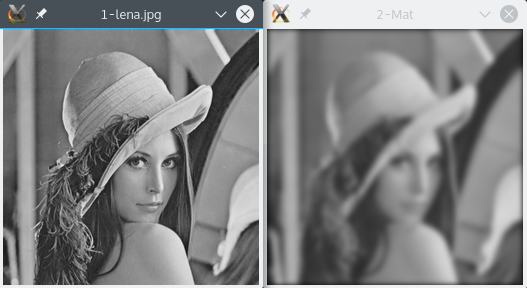
\includegraphics[width=0.7\textwidth]{LenaConv.png}}


  \section{Imágenes Híbridas}

  Una imagen híbrida es una \"mezcla\" de dos imágenes, donde de una tomamos las altas
  frecuencias y de la otra las bajas. Al unirlas, podemos lograr el efecto de
  ver una de ellas mientras estemos cerca y la otra si miramos desde lejos.\\

  Utilizando el filtro Gaussiano conseguimos funciones para generar imágenes de alta
  y baja frecuencia,

  [Insertar código, HAY QUE HACERLO, LO HE HECHO MAL]

  Las sumamos y conseguimos este resultado

  \centerline{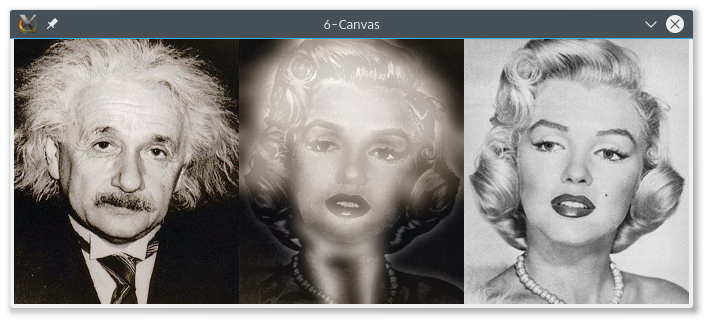
\includegraphics[width=0.7\textwidth]{Hybrid.png}}

  \section{Pirámide Gaussiana}

  Para realizar la pirámide, no tenemos más que realizar un \textit{downsampling}
  a la imagen. Para ello hemos realizado este pequeño bonus implementando el
  \textit{downsampling}, y no usando \textit{pyrDown()}.\\

  Tomando 2 índices para cada imagen, es fácil quitarnos las filas y columnas pares.
  Es importante, como hemos visto en teoría, alisar antes la imagen. Tomamos $\sigma=1$
  para que sean 3 píxeles los que se miren. No tiene sentido hacerlo mayor, ya que
  vamos a quitar muchos píxeles vecinos.

  \begin{lstlisting}
    Image Image::downsample()
    {
      // Classic technique: Blur and downsample (deleting odd cols and rows)
      Mat output = Mat::zeros(image.rows / 2, image.cols / 2, image.type());

      int i1, i2;
      int j1, j2;

      Mat mask = gaussianMask(1);
      Mat image_blur = convolution2D(image,mask,false);

      if (image.channels() == 1)
      {
        for (i1 = 0, i2 = 0; i1 < image_blur.rows && i2 < output.rows; i1+=2, i2++)
          for (j1 = 0,j2 = 0; j1 < image_blur.cols && j2 < output.cols; j1+=2,j2++)
            output.at<float>(Point(j2,i2)) = image_blur.at<float>(Point(j1,i1));
      }
      else
      {
        for (i1 = 0, i2 = 0; i1 < image_blur.rows && i2 < output.rows; i1+=2, i2++)
          for (j1 = 0,j2 = 0; j1 < image_blur.cols && j2 < output.cols; j1+=2,j2++)
            output.at<Vec3b>(Point(j2,i2)) = image_blur.at<Vec3b>(Point(j1,i1));
      }

      return Image(output);
    }
  \end{lstlisting}

  Después de aplicar esto varias veces, insertamos los resultados
  en el mismo canvas y obtenemos el curioso resultado.

  \centerline{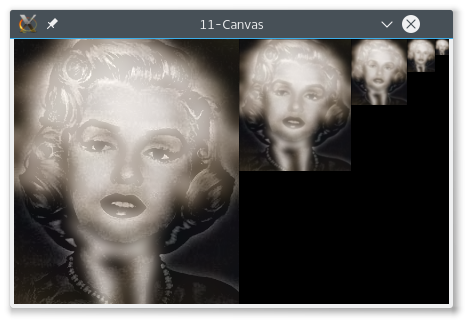
\includegraphics[width=0.7\textwidth]{HybridPyramid.png}}

  \section{Bonus 1}

  Se ha implementado una función que calcula 2 máscaras para las parciales en $X$ e $Y$
  de la Gaussiana. Recordando las parciales:

  \[
   \frac{\partial G}{\partial x} = - \frac{x e^{- \frac{x^{2}}{2 \sigma^{2}}}}{\sqrt{2 \pi} \sigma^{2}} \frac{e^{- \frac{y^{2}}{2 \sigma^{2}}}}{\sqrt{2 \pi} \sigma^{2}}
  \]

  Y para la derivada en $y$,

  \[
   \frac{\partial G}{\partial y} = - \frac{e^{- \frac{x^{2}}{2 \sigma^{2}}}}{\sqrt{2 \pi} \sigma^{2}} y\frac{e^{- \frac{y^{2}}{2 \sigma^{2}}}}{\sqrt{2 \pi} \sigma^{2}}
  \]

  Explico: la primera parte del cómputo es para el operando que tiene a la propia
  variable multiplicando (para la parcial en $X$, por ejemplo, el primer operando).
  La segunda es para el otro, claramente. Como son simétricos, calculamos ambas
  y al final comprobamos el eje: Si es el $X$, tomamos la parcial en $X$ (en el orden
  arriba indicado) y en otro caso la de $Y$.

  \begin{lstlisting}
    vector <Mat> Image::MaskFirstDerivative(float sigma, char axis)
    {
      int mask_size = 2 * round(3 * sigma) + 1; // +-3*sigma plus the zero
      int mask_center = round(3 * sigma);

      float value = 0, sum_values = 0;
      int mask_index;

      Mat mask_x = Mat::zeros(1, mask_size, CV_32FC1);

      for (int i = 0; i < mask_size; i++)
      {
        mask_index = i - mask_center;
        value = -mask_index * exp(-0.5 * (mask_index * mask_index) / (2*sigma * sigma)) * sqrt(0.5);

        mask_x.at<float>(Point(i,0)) = value;
        sum_values += value;
      }

      mask_x *= 1.0 / sum_values;

      // The another part

      value = 0;
      sum_values = 0;

      Mat mask_1 = Mat::zeros(1, mask_size, CV_32FC1);

      for (int i = 0; i < mask_size; i++)
      {
        mask_index = i - mask_center;
        value = - exp(-0.5 * (mask_index * mask_index) / (2*sigma * sigma)) * sqrt(0.5);

        mask_1.at<float>(Point(i,0)) = value;
        sum_values += value;
      }

      mask_1 *= 1.0 / sum_values;

      vector <Mat> derivatives;
      if (axis == "x")
      {
        derivatives.push_back(mask_x);
        derivatives.push_back(mask_1);
      }
      else
      {
        derivatives.push_back(mask_1);
        derivatives.push_back(mask_x);
      }

      return derivatives;
    }
  \end{lstlisting}

  Para hacer la prueba se ha utilizado otra función

  \begin{lstlisting}
    Image Image::calcFirstDerivative(float sigma, char axis, bool reflected)
    {
      vector<Mat> derivatives = MaskFirstDerivative(sigma,axis);
      Mat mask = derivatives[0].clone();

      flip(mask,mask,-1);

      // First we blur the image
      Image tmp = GaussConvolution(3,true);

      Mat output = tmp.image.clone();


      // Convolution
      for (int i = 0; i < output.rows; i++)
      {
        Mat row = output.row(i).clone();
        convolution1D(row,mask,reflected).copyTo(output.row(i));
      }

      // Transposing for convolution by cols
      output = output.t();

      mask = derivatives[1].clone();
      flip(mask,mask,-1);

      for (int i = 0; i < output.rows; i++)
      {
        Mat row = output.row(i).clone();
        convolution1D(row,mask,reflected).copyTo(output.row(i));
      }
      // Re-transposing to make the correct image
      output = output.t();

      return Image(output);
    }
  \end{lstlisting}

  Aquí muestro una salida con la foto de Einstein.

  \centerline{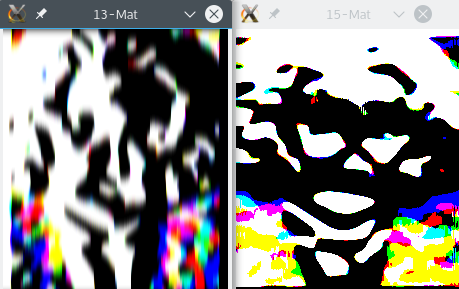
\includegraphics[width=0.7\textwidth]{Derivative.png}}

  \section{Bonus 2}

  El segundo bonus consiste en, usando las funciones de OpenCV, utilizar el filtro
  Canny en una imagen y mostrarlo sobre color sólido. Se muestra aquí la función
  implementada. Tomamos $\sigma=3$ para el alisamiento ya que el filtro de Canny
  tiene un kernel de $3\times3$ por defecto.

  \begin{lstlisting}
    Image Image::detectEdges(double lowThreshold, double highThreshonld)
    {
      // First of all we blur the image
      Image tmp = GaussConvolution(3,true);

      Mat edges;

      // Apply Canny filter!
      Canny(tmp.image, edges, lowThreshold, highThreshonld);

      // Black background
      Mat dest = Mat::zeros(tmp.image.rows, tmp.image.cols, tmp.image.type());

      // Copy the input image to dest using the edges as mask
      tmp.image.copyTo(dest, edges);

      return Image(dest);
    }
  \end{lstlisting}

  Aquí muestro un ejemplo con la foto de la bicicleta. Se han tomado los valores
  40 y 60 como valores de threshold de manera empírica, teniendo en cuenta que
  en esta ocasión quería la silueta de la bicicleta, pero intentando eliminar los
  radios de las ruedas. En la rueda de delante no han desaparecido todos por completo,
  pero en la de atrás el resultado es muy bueno.


  \centerline{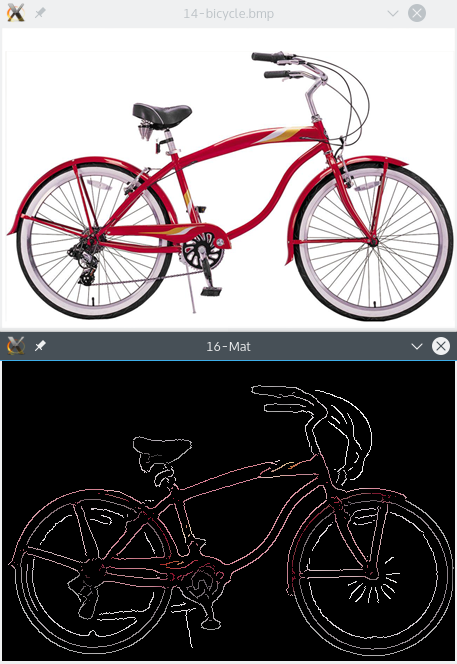
\includegraphics[width=0.7\textwidth]{Canny.png}}

  Y por último, aquí muestro el fichero main con las llamadas

  \begin{lstlisting}
    #include "../inc/image.hpp"
    #include "../inc/utils.hpp"
    #include <iostream>

    using namespace std;
    using namespace cv;

    int main(int argc, char const *argv[]) {
      Image lena(string("imagenes/lena.jpg"),false);
      Image lena_conv = lena.GaussConvolution(3);
      lena.paint();
      lena_conv.paint();

      waitKey(0);
      destroyAllWindows();

      Image einstein(string("imagenes/einstein.bmp"),true);
      Image marilyn(string("imagenes/marilyn.bmp"),true);

      Image hybrid = einstein.createHybrid(marilyn,true,6,6);

      vector<Image*> secuencia;
      secuencia.push_back(&einstein);
      secuencia.push_back(&hybrid);
      secuencia.push_back(&marilyn);

      Image tira(secuencia,1,3);
      tira.paint();

      waitKey(0);
      destroyAllWindows();

      vector<Image*> pyramid;
      Image hybrid_d1 = hybrid.downsample();
      Image hybrid_d2 = hybrid_d1.downsample();
      Image hybrid_d3 = hybrid_d2.downsample();
      Image hybrid_d4 = hybrid_d3.downsample();
      pyramid.push_back(&hybrid);
      pyramid.push_back(&hybrid_d1);
      pyramid.push_back(&hybrid_d2);
      pyramid.push_back(&hybrid_d3);
      pyramid.push_back(&hybrid_d4);

      Image pyramidImage(pyramid, 1,5);

      pyramidImage.paint();

      waitKey(0);
      destroyAllWindows();

      Image derivative_x = einstein.calcFirstDerivative(3,"x");
      Image derivative_y = einstein.calcFirstDerivative(3,"y");
      derivative_x.paint();
      derivative_y.paint();

      waitKey(0),
      destroyAllWindows();

      Image bicycle(string("imagenes/bicycle.bmp"),true);
      Image edges_bicycle = bicycle.detectEdges(40,60);

      bicycle.paint();
      edges_bicycle.paint();

      waitKey(0);
      destroyAllWindows();

      return 0;
    }
  \end{lstlisting}




\end{document}
